\documentclass[a4paper]{article}
\usepackage[spanish]{babel}
\usepackage[utf8]{inputenc}
\usepackage{graphicx}
\usepackage{biblatex}
\usepackage{enumerate}
\usepackage{csquotes}
\usepackage{braket}
\usepackage{amsmath}
\addbibresource{bibliografia.bib}

\title{Modos rotacionales y vibracionales en moléculas}
\author{José Soto García}
\begin{document}
\maketitle

\section{La molécula como un sólido rígido: hamiltoniano asociado a la rotación de la misma en torno a su centro de masas.}
Un sólido rígido se define como una colección de partículas, cuyas distancias relativas se mantienen fijas \cite{marion2013}. Dado que la distancia es fija, la energía potencial no varía con la rotación del rotor, luego $V=0$. El momento de inercia $I_i$ de un sólido rígido con $n$ partículas sobre un eje $i$ se define como:
\begin{equation}
I_i= \sum_{j=1}^n=m_jr_j^2
\end{equation}
con $r_j$ la distancia desde la partícula de masa $m_j$ al eje $i$.

Para un sólido poliatómico, se define el tensor de inercia $\tilde{I}$ como:
\begin{equation}
\tilde{I}=\begin{pmatrix}
\displaystyle\sum_{\alpha}m_{\alpha}\left(x^2_{\alpha,2}+x^2_{\alpha,3}\right) & -\displaystyle\sum_{\alpha}m_{\alpha}x_{\alpha,1}x_{\alpha,2} & -\displaystyle\sum_{\alpha}m_{\alpha}x_{\alpha,1}x_{\alpha,3} \\\\
-\displaystyle\sum_{\alpha}m_{\alpha}x_{\alpha,2}x_{\alpha,1} & \displaystyle\sum_{\alpha}m_{\alpha}\left(x^2_{\alpha,1}+x^2_{\alpha,3}\right) &-\displaystyle\sum_{\alpha}m_{\alpha}x_{\alpha,2}x_{\alpha,3} \\\\
-\displaystyle\sum_{\alpha}m_{\alpha}x_{\alpha,3}x_{\alpha,1} & -\displaystyle\sum_{\alpha}m_{\alpha}x_{\alpha,3}x_{\alpha,2} & \displaystyle\sum_{\alpha}m_{\alpha}\left(x^2_{\alpha,1}+x^2_{\alpha,2}\right) \end{pmatrix}
\end{equation}
Clásicamente, la energía cinética rotacional del sistema se obtiene como:
\begin{equation}
T_{rot}=\frac{1}{2}\sum_{i,j}I_{i,j}\omega_i\omega_j
\end{equation}
Una clara simplificación se encuentra si diagonalizamos el tensor de inercia. Los vectores que diagonalizan la matriz de inercia son los denominados ejes principales de inercia. La energía cinética rotacional clásica del sistema queda por tanto \cite{marion2013}:
\begin{equation}
T_{rot}=\frac{1}{2}\left(I_a\omega^2_a + I_b\omega^2_b + I_c\omega^2_c\right) 
\end{equation}
con $I_a$, $I_b$, e $I_c$ los autovalores del momento de inercia.\\
Los ejes principales de inercia normalmente se toman de forma que
\begin{equation}
I_a \leq I_b \leq I_c
\end{equation}

Para formar el hamiltoniano del sistema, necesitamos la energía en función del momento angular $P$, con $P_i=I_i\omega_i$.
La energía cinética queda entonces como:
\begin{equation}
T_{rot}=\frac{P_a^2}{2I_a}+\frac{P_b^2}{2I_b}+\frac{P_c^2}{2I_c}
\end{equation}
Una vez tenemos la energía cinética en función de los momentos angulares debemos sustituir los momentos angulares $P_i$ por su operador correspondiente cuántico $\hat P_i$.\\

El nuevo sistema de referencia $\left\lbrace a,b,c \right\rbrace$ se consigue mediante tres rotaciones  $\left\lbrace \theta,\phi,\chi \right\rbrace$ a través del centro de masas $O$. Son los llamados ángulos de Euler (figura \ref{euler}).
De la figura \ref{euler} podemos ver que:
\begin{equation}
\hat P_{\phi}=-i\hbar\frac{\partial}{\partial \phi},\,\ \hat P_{N}=-i\hbar\frac{\partial}{\partial N},\,\ \hat P_{\chi}=-i\hbar\frac{\partial}{\partial \chi}
\end{equation}

\begin{figure}
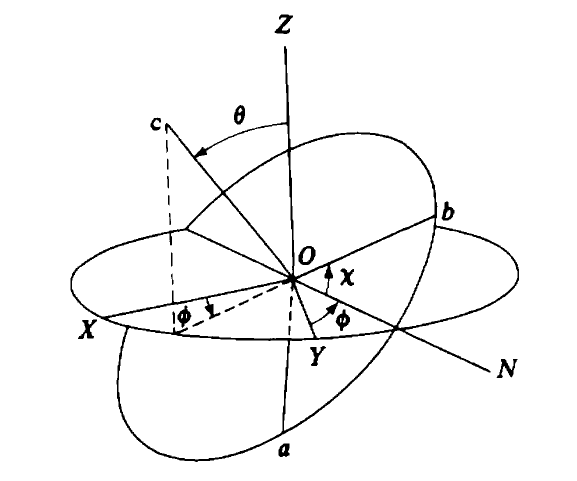
\includegraphics[width=0.8\textwidth]{Angulos_Euler.png}
\caption{Ángulos de Euler. $ON$ es la línea de intersección de los planos $XY$ y $ab$, y es perpendicular a los ejes $OZ$ y $Oc$. $\theta$ es el ángulo de rotación sobre el eje $ON$; $\phi$ es el ángulo de rotación sobre el eje $OZ$; $\chi$ es el ángulo de rotación sobre el eje $Oc$ }
\label{euler}
\end{figure}

Teniendo en cuenta que 

$$ P_N=  P_a sin\chi + P_b cos\chi$$  
$$ P_Z= -P_a sin\theta cos\chi + P_b sin\theta sin\chi + P_c cos\theta $$

Obtenemos que:

\begin{equation}
\hat P_a = i\hbar \left[cos\chi csc\theta \frac{\partial}{\partial \phi} - cos\chi cot\theta \frac{\partial}{\partial \chi} - sin\chi \frac{\partial}{\partial \theta} \right]
\end{equation}
\begin{equation}
\hat P_b = i\hbar \left[-sin\chi csc\theta \frac{\partial}{\partial \phi} + sin\chi cot\theta \frac{\partial}{\partial \chi} - cos\chi \frac{\partial}{\partial \theta} \right]
\end{equation}
\begin{equation}
\hat P_c = -i\hbar \frac{\partial}{\partial\chi}
\end{equation}
O también:

\begin{equation}
\hat P_X = i\hbar \left[cos\phi cot\theta \frac{\partial}{\partial \phi} - cos\phi csc\theta \frac{\partial}{\partial \chi} + sin\phi \frac{\partial}{\partial \theta} \right]
\end{equation}
\begin{equation}
\hat P_Y = i\hbar \left[sin\phi cot\theta \frac{\partial}{\partial \phi} - sin\phi csc\theta \frac{\partial}{\partial \chi} - cos\phi \frac{\partial}{\partial \theta} \right]
\end{equation}
\begin{equation}
\hat P_Z = -i\hbar\frac{\partial}{\partial\phi} 
\end{equation}

Sabemos que el hamiltoniano rotacional es
\begin{equation}
\hat H_{rot}=\frac{\hat P_a^2}{2I_a}+\frac{\hat P_b^2}{2I_b}+\frac{\hat P_c^2}{2I_c}
\end{equation}
y el operador momento angular total es:
\begin{equation}
\hat P^2 = \hat P_a^2+  \hat P_b^2+  \hat P_c^2 = \hat P_X^2+  \hat P_Y^2+  \hat P_Z^2
\end{equation}
Una forma de obtener los autovalores de Energía sería sustituir los valores de $\hat P_a$, $\hat P_b$ y $\hat P_c$ en el hamiltoniano $\hat H_{rot}$ y resolver la ecuación de autovalores. Sin embargo, estos autovalores se pueden obtener mediante relaciones de conmutación.
Las relaciones de conmutación que necesitaremos son las siguientes:
\begin{equation}
\left[\hat P_i,\hat P_j\right]=-i\hbar\delta_{i,j}\hat P_k
\end{equation}
\begin{equation}
\left[\hat P_I,\hat P_J\right]=i\hbar\delta_{I,J}\hat P_K
\end{equation}
\begin{equation}
\left[\hat P^2,\hat P_j\right]=\left[\hat P^2,\hat P_J\right]=0
\end{equation}
\begin{equation}
\left[\hat P_J,\hat P_j\right]=0 \,,\ \forall_{J,j}
\end{equation}
con $J = \left\lbrace X,Y,Z \right\rbrace$ y $j= \left\lbrace a,b,c \right\rbrace$ \\
Con estas relaciones de conmutación es fácil comprobar que:
\begin{equation}
\left[H_{rot}, \hat P^2 \right] = 0
\end{equation}
\begin{equation}
\left[H_{rot}, \hat P_J \right] = 0
\end{equation}
\begin{equation}
\left[H_{rot}, \hat P_c \right] = i\hbar \left(\frac{1}{2I_a}-\frac{1}{2I_b}\right)\left(\hat{P_a}\hat{P_b}+\hat{P_b}\hat{P_a}\right)
\end{equation}
Puesto que $H_{rot}$ conmuta con $\hat{P^2}$ y con $\hat P_Z$,  se pueden elegir las autofunciones $\psi$ del hamiltoniano rotacional como autofunciones de ambos operadores. Además, como los operadores $\hat P_X, \,\ \hat P_Y \,\ y \,\ \hat P_Z$ cumplen las relaciones generales de conmutación del momento angular, obtenemos las siguientes relaciones:
\begin{equation}
\hat H\psi = E\psi
\end{equation}
\begin{equation}
\hat P^2\psi = J(J+1)\hbar \psi, \qquad J=0,1,2...
\end{equation}
\begin{equation}
\hat P_Z\psi = M\hbar\psi, \qquad M = 0,\pm 1,...,\pm J
\end{equation}
y las autofinciones del rotor son de la forma:
\begin{equation}
\psi = F(\theta, \psi)(2\pi)^{-1/2}e^{iM\phi}
\end{equation}
Los autovalores de energía dependerán de las simetrías de rotación que presente la molécula. Estas simetrías pueden ser:\\
Rotor esférico $I_a=I_b=I_c= I$ \\
Rotor simétrico $I_a=I_b \neq I_c$ o $I_a\neq I_b=I_c$\\
Rotor asimétrico $I_a \neq I_b \neq I_c$\\
\section{Rotor rígido cuántico: Estados propios y autovalores.}
\subsection{El rotor esférico}
El rotor esférico se caracteriza porque los tres momentos principales de inercia son iguales: $$I_a=I_b=I_c= I$$
El hamiltoniano del sistema queda por tanto como:
\begin{equation}
\hat H = \frac{\hat P^2}{2I}
\end{equation}
La ecuación de Schödinger es:
\begin{equation}
\frac{\hat P^2}{2I} \psi = E\psi
\end{equation}
Resolviendo la ecuación obtenemos que:$$\frac{1}{2I}J(J+1)\hbar^2\psi=E\psi$$
\begin{equation}
E=\frac{J(J+1)\hbar^2}{2I}, \qquad J=0,1,2...
\end{equation}
En este caso, tenemos además que
\begin{equation}
\left[\hat H,\hat P_c \right]=0
\end{equation}
con $$\hat P_c \psi = K\hbar\psi, \qquad K = 0, \pm 1,..., \pm J$$
Luego la energía está $(2J+1)^2$ veces degenerada.
\subsection{El rotor simétrico}
El rotor simétrico se caracteriza porque dos de sus momentos principales de inercia son iguales $I_a=I_b\neq I_c$ (caso achatado) o $I_a\neq I_b=I_c$ (caso alargado). Realizaremos el desarrollo del caso $I_a=I_b\neq I_c$ y luego lo adaptaremos al caso alargado. 
El hamiltoniano del sistema es:
\begin{equation}
\hat H=\frac{\hat P_a^2+\hat P_b^2}{2I_b}+\frac{\hat P_c^2}{2I_c}=\frac{\hat P^2- \hat P_c^2}{2I_b}+\frac{\hat P_c^2}{2I_c}
\end{equation}
Como $\hat P_c$ conmuta con $\hat P^2$ y con $\hat P_c^2$, el hamiltoniano conmuta con $\hat P_c$, y las autofunciones del hamiltoniano se pueden elegir como autofunciones de $\hat P_c$.
Las energías se obtienen como: $$\left(\frac{\hat P^2- \hat P_c^2}{2I_b}+\frac{\hat P_c^2}{2I_c}\right)\psi=E\psi$$
 $$\left(\frac{\hbar^2J(J+1)- \hbar^2K^2}{2I_b}+\frac{\hbar^2K^2}{2I_c}\right)\psi=E\psi$$
 Luego:
 \begin{equation}
 E=\frac{\hbar^2J(J+1)}{2I_b}+\hbar^2K^2\left(\frac{1}{2I_c}-\frac{1}{2I_b}\right)
 \end{equation}
 Se definen las constantes rotacionales como:
 \begin{equation}
 A \equiv \frac{h}{8\pi^2I_a}\geq B\equiv \frac{h}{8\pi^2I_b}\geq C\equiv \frac{h}{8\pi^2I_c}
 \end{equation}
 Y las energías son por tanto:
 \begin{equation}
 E/h=BJ\left(J+1\right)+\left(C-B\right)K^2 \qquad (achatado)
 \end{equation}
 \begin{equation}
 E/h=BJ\left(J+1\right)+\left(A-B\right)K^2 \qquad (alargado)
 \end{equation}
La energía depende de $J$ y $K^2$. Hay una degeneración $(2J+1)$ asociada a $M$. Además, para $K\neq 0$ hay una degeneración doble debida a los valores de $\pm K$, luego para $K\neq 0$ la degeneración de la energía es $4J+2$.
\subsection{El rotor asimétrico}
En el rotor asimétrico $I_a\neq I_b\neq I_c$
En este caso, como $\left[\hat H,\hat P_c\right]\neq 0$ no podemos elegir las autofunciones de $\hat P_c$; además el hamiltoniano no es separable y necesitaremos otro método para resolver la ecuación de Schrödinger.\\
Podemos  encontrar los autovalores de $\hat H$ expandiendo las autofunciones desconocidas $\psi_i$ en términos de algún conjunto completo ortonormal conocido $\phi_i$ y resolviendo la ecuación de autovalores:
\begin{equation}
det \left[ \bra{\phi_n}\hat H\ket{\phi_m} - E_i\delta_{nm} \right]=0
\end{equation}
Un conjunto completo ortonormal que podemos usar son las autofunciones del rotor simétrico, ya que son funciones de las mismas coordenadas (los ángulos de Euler) y satisfacen las mismas condiciones de contorno:
\begin{equation}
\psi_i = \sum_{J'}\sum_{M'}\sum_{K'}c_{i,J'M'K'}\phi_{J'M'K'}
\end{equation}
Como $\psi_i$ es autofunción de $\hat P^2$ con autovalor $\hbar^2J(J+1)$ y de $\hat P_z$ con autovalor $\hbar M$ sólo necesitamos incluir fuciones $\phi_i$ con el mismo valor de $J$ y $M$ que $\psi_i$. La suma infinita sobre $J'$, $M'$ y $K'$ se reduce ahora a una suma finita sobre los $2J+1$ posibles valores de $K'$
\begin{equation}
\psi_i = \sum_{K'=-J}^Jc_{i,JMK'}\phi_{JMK'}
\end{equation}
Luego, la ecuación de autovalores queda:
\begin{equation}
det\left(H_{K'K''}-E_i\delta_{K'K''}\right)=0
\end{equation}
con
\begin{equation}
H_{K'K''}\equiv\int\phi^*_{JMK'}\hat H\phi_{JMK''}d\tau
\end{equation}
Cuyo resultado es calculable con los datos que tenemos y vale:
$$
H_{K'K''}=\delta_{K''K'}\frac{1}{2}h\left[\left(2C-A-B\right)\left(K'\right)^2+\left(A+B\right)J\left(J+1\right)\right]$$$$+\delta_{K''K'+2}\frac{1}{4}h\left(B-A\right)\left[J\left(J+1\right)-K'\left(K'+1\right)\right]^\frac{1}{2}$$$$\cdot\left[J\left(J+1\right)-\left(K'+1\right)\left(K'+2\right)\right]^\frac{1}{2}$$$$+\delta_{K''K'-2}\frac{1}{4}h\left(B-A\right)\left[J\left(J+1\right)-K'\left(K'-1\right)\right]^\frac{1}{2}$$
\begin{equation}
\cdot\left[J\left(J+1\right)-\left(K'-1\right)\left(K'-2\right)\right]^\frac{1}{2}
\end{equation}
Siendo
$$
A \equiv \frac{h}{8\pi^2I_a}\geq B\equiv \frac{h}{8\pi^2I_b}\geq C\equiv \frac{h}{8\pi^2I_c}
$$
Las primeras energías son, en orden creciente:\\
Para $J = 0$
$$E = 0$$
Para $J = 1$
$$E = h(B+C), \,\ h(A+C), \,\ h(A+B)$$
Podemos ver que los autovalores del hamiltoniano no dependen de $M$, por tanto, la degeneración de la energía será $2J+1$, correspondiente a los posibles valores de $M$ para un $J$ dado.
Cada función de onda del rotor asimétrico $\psi_i$ es una combinación lineal de las $2J+1$ funciones de onda de del rotor simétrico con los mismos valores de $J$ y $M$ que $\psi_i$.
\subsection{El rotor rígido diatómico}
El rotor rígido de dos partículas puede considerarse como un caso especial del rotor rígido simétrico en el que $I_a = 0$ y por tanto $K=0$. Consiste en dos masas $m_1$ y $m_2$ unidas a una barra sin masa con una distancia fija $d$. El momento de inercia de una molécula diatómica puede escribirse como:
\begin{equation}
I=\mu R^2
\end{equation}
Podemos determinar los niveles de energía de este sistema resolviendo la ecuación de Schrödinger. Suponiendo que el radio entre los dos átomos no varía, la ecuación de Schrödinger queda:
\begin{equation}
- \frac{\hbar^2}{2I}\left[\frac{1}{sin\theta}\frac{\partial}{\partial \theta}\left(sin\theta \frac{\partial}{\partial \theta} \right) + \frac{1}{sin^2\theta}\frac{\partial^2}{\partial \phi^2}\right]Y^m_l \left(\theta,\phi \right) = E_lY^m_l \left(\theta,\phi \right)
\end{equation}
Con
$$E_l= \frac{\hbar^2}{2I}l(l+1)$$
Si llamamos $$B\equiv \frac{h}{8\pi^2I}$$
obtenemos que:
\begin{equation}
E/h=BJ(J+1)
\end{equation}
La energía está $2l+1$ veces degenerada debido a que para un $l$ fijo, distintos valores de $m$ tienen la misma energía.

\section{Estructura del espectro rotacional.}
El espectro rotacional de las moléculas se observa casi exclusívamente como espectro de absorción, ya que la emisión espontánea es muy poco probable dada las bajas energías de transición. El espectro rotacional cae en la región de las microondas, por lo que se requieren espectrómetros del infrarojo lejano o espectrómetros de microondas para observarlos.\cite{haken2013}\\

Sólo las moléculas con momento dipolar eléctrico permanente permiten la observación de su espectro rotacional.  Esto es debido a que este tipo de moléculas, cuando está rotando, parece tener un momento dipolar dependiente del tiempo para un observador estacionario. La rotación de este tipo de moléculas lleva absorción de radiación electromagnética cuando las frecuencia electromagnética irradiada encaja con la frecuencia de rotación del dipolo. Por tanto, moléculas homonucleares diatómicas como el $H_2$, el $N_2$ o el $O_2$ no presentan espectro rotacional. Lo mismo ocurre con moléculas más grandes como el $CCl_4$, a menos que la rotación induzca un momento dipolar o la molécula presente algún tipo de vibración asimétrica que le induzca un momento \cite{haken2013}.\\
 
Los elementos diagonales del operador $\hat D$ dados por:
\begin{equation}
D_{\alpha\alpha}=\bra{\psi_\alpha}\hat D\ket{\psi_\alpha},\qquad \alpha \equiv \left(s,v,J,M,K\right),
\end{equation}
determinan el momento dipolar eléctrico permanente de la molécula en el estado $\psi_\alpha$.\\

Las reglas de selección que aparecen asociadas a las transiciones electromagnéticas en moléculas son las habituales para una transición dipolar eléctrica, esto es, son las que corresponden al valor esperado de un tensor esférico de primer orden entre estados de momento angular definido.
Para el rotor simétrico tenemos como reglas de selección
\begin{equation}
\Delta J = 0,\pm 1 \qquad\Delta K =0 \qquad \Delta M = 0, \pm 1
\end{equation}
Teniendo que cuando $\Delta J = 0$ con $\Delta M \neq 0$ no hay absorción o emisión de radiación.\\

Para el caso más simple, esto es una molécula heteronuclear diatómica, tenemos que 
\begin{equation}
h\nu = E_{J+1}-E_{J}
\end{equation}
Luego
\begin{equation}
\nu_{J \rightarrow J+1} = 2B(J+1)
\end{equation}
De esta ecuación podemos observar que moléculas más pesadas, las cuales tendrán un $I$ mayor y por tanto una constante rotacional $B$ menor, tendrán un espaciado menor entre sus líneas de absorción (figura \ref{niveles1}).
\begin{figure}
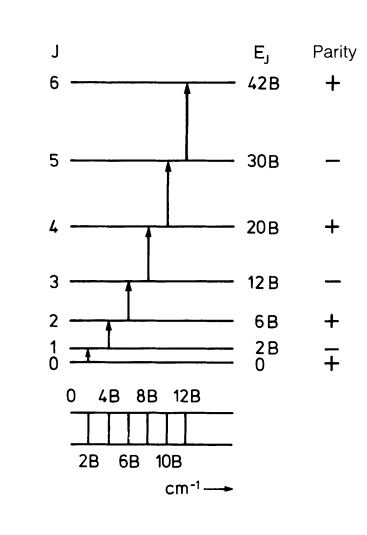
\includegraphics[width=0.6\textwidth]{niveles1.png}
\caption{Niveles energéticos para la rotación de una molécula diatómica rígida. La paridad de los niveles queda a la derecha de la figura, podemos observar que la regla de selección implica un cambio en la paridad de la molécula.}
\label{niveles1}
\end{figure}
\section{Momentos de inercia de distintas moléculas respecto de sus ejes principales en sus estados fundamentales: $H_2$ , $CO$, $H_2O$ , $CH_4$ ...}
En esta sección  para simplificar los cálculos trabajaremos con unidades naturales, es decir tomaremos $\hbar = 1$ y $c=1$.
Las constantes rotacionales las escribiremos como:
$$A' = \frac{1}{2I_a}$$
\subsection{$H_2$}
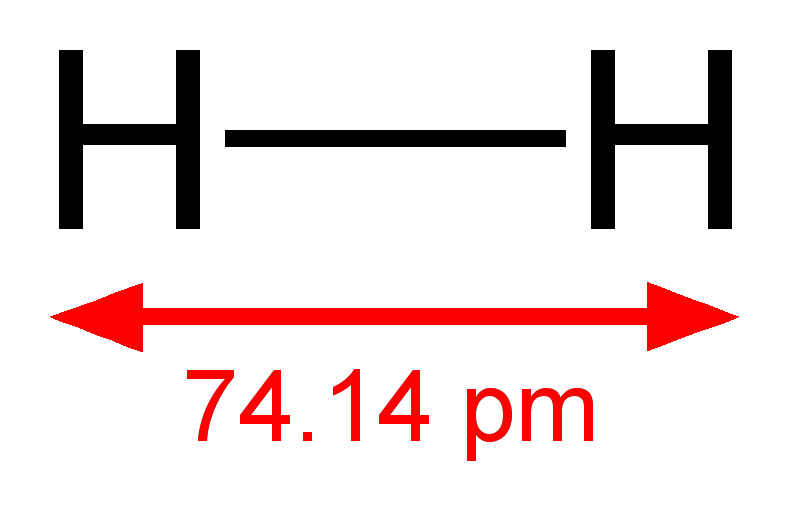
\includegraphics[width=0.3\textwidth]{hidrogeno.png}\\
La molécula de hidrógeno $(H_2)$ es una molécula diatómica homonuclear. Su momento de inercia puede calcularse como $$I=\mu R^2$$
como $m_1=m_2=m$ tenemos entonces que $$I=\frac{1}{2}mR^2$$
Teniendo que\\
 $R=74 \, pm=375.014 \, MeV^{-1}$\\
 $m=938.272 \, MeV/c^2$\\
 
 Nos queda que $$I=65.977 \, eV^{-1}c^{-2}$$
 luego 
 $$B'=7.58\cdot 10^{-3}\, eV$$
 Y
 $$E_{rot} = 7.58\cdot 10^{-3}J(J+1)\, eV$$
 \subsection{$CO$}
 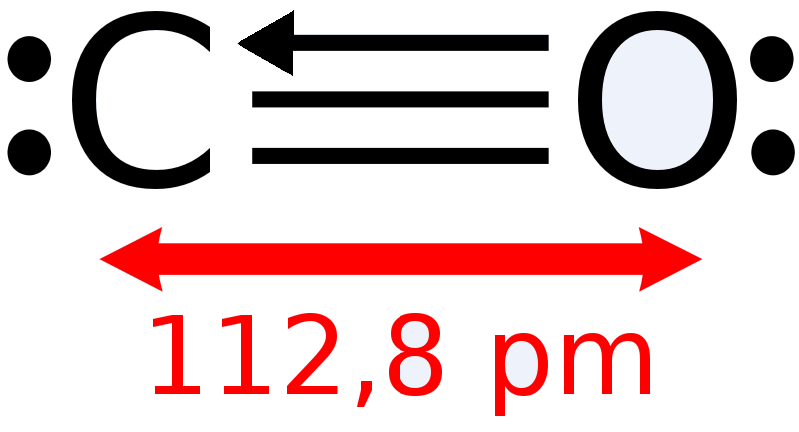
\includegraphics[width=0.3\textwidth]{monoxido.png}\\
 La molécula de monóxido de carbono $(CO)$ es una molécula diatómica heteronuclear. Su momento de inercia, como en el caso anterior es $$I=\mu R^2$$
 $R=112.8 \, pm=571.642\, MeV^{-1}$\\
 $m_c=12.0107 \, u=11\, 187.97 \, MeV/c^2$\\
 $m_0=15.999\, u=14\, 903.069\, MeV/c^2$\\
 En este caso 
 $$I= 2\, 088.335\,eV^{-1}c^{-2}$$
 Luego
 $$B'=2.4 \cdot 10^{-4} \, eV$$
 Y la energía por tanto
 $$E_{rot} =2.4 \cdot 10^{-4} J(J+1)\, eV$$
 \subsection{$H_2O$}
 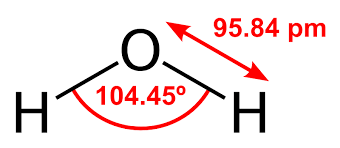
\includegraphics[width=0.4\textwidth]{agua.png}\\
 Las posiciones de los átomos de agua $(H_2O)$ respecto a su centro de masas son:\\
 $\vec r_O = 0\, \vec x + 33.29 \, \vec y + 0 \, \vec z \, MeV^{-1}$\\
 $\vec r_{H1} =-383.94\, \vec x-264.24 \, \vec y + 0 \, \vec z \, MeV^{-1}$\\
 $\vec r_{H2} = 383.94 \, \vec x -264.24 \, \vec y + 0 \, \vec z \, MeV^{-1}$\\
 
 Y las masas de los átomos son\\
 $M_H = 938.272 \, MeV$\\
 $M_O = 14\, 903.069 MeV$\\
 
 A partir de ellos construimos su tensor de inercia
 $$ \tilde I =
 \begin{pmatrix}
 147.546 & 0 & 0 \\
 0 & 276.621 & 0 \\
 0 & 0 & 424.167\\
 \end{pmatrix}
 \, eV^{-1}
 $$
 Vemos que el tensor de inercia es diagonal en las coordenadas cartesianas. Por lo que sus ejes principales son $ \hat x, \,\ \hat y, \,\ \hat z$\\
 En este caso tenemos un rotor asimétrico. Donde:
 $$A'= 3.4 \cdot 10^{-3}\, eV \qquad B' = 1.8 \cdot 10^{-3}\, eV \qquad C' = 1.2 \cdot 10^{-3}\, eV$$
 Las primeras energías son:
 $$E_0 = 0$$
 $$E_1 = (B'+C') = 3 \cdot 10^{-3}\, eV $$
 $$E_2 = (A'+C') = 4.6 \cdot 10^{-3}\, eV$$
 $$E_3 = (A'+B') = 5.2 \cdot 10^{-3}\, eV$$ 
 \subsection{$CH_4$}
 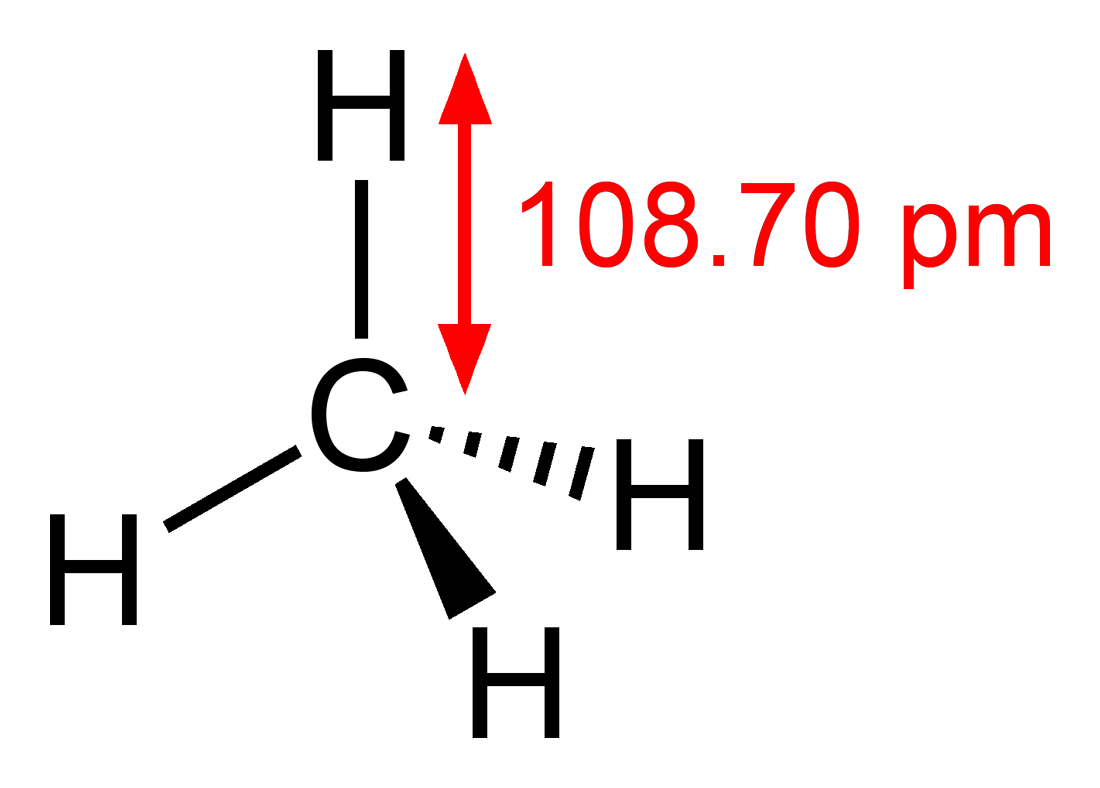
\includegraphics[width=0.4\textwidth]{metano.png}\\
Las posiciones de los átomos  de metano $(CH_4)$ respecto a su centro de masas son:
 $\vec r_C = 0\, \vec x + 0 \, \vec y + 0 \, \vec z \, MeV^{-1}$\\
 $\vec r_{H1} = 0\, \vec x+0 \, \vec y + 550.87 \, \vec z \, MeV^{-1}$\\
 $\vec r_{H2} = 0\, \vec x -477.1 \, \vec y + -275.4\, \vec z \, MeV^{-1}$\\
 $\vec r_{H3} = 413.2\, \vec x + 238.5 \, \vec y + -272.4 \, \vec z \, MeV^{-1}$\\
 $\vec r_{H4} = -413.2 \, \vec x -238.5 \, \vec y + -272.4 \, \vec z \, MeV^{-1}$\\
 
 Y las masas de los átomos son\\
 $M_C = 11\, 187.97 \, MeV$\\
 $M_H = 938.272 MeV$\\
 
 A partir de estos datos construimos el tensor de inercia
 $$ \tilde I =
 \begin{pmatrix}
 818.6 & 0 & 0 \\
 0 & 818.6 & 0 \\
 0 & 0 & 640.7\\
 \end{pmatrix}
 \, eV^{-1}
 $$
 
Los ejes principales son también los ejes cartesianos $ \hat x, \,\ \hat y, \,\ \hat z$. 
Esta molécula se comporta rotor simétrico alargado, con 
 $$A'= 7.7 \cdot 10^{-3}\, eV \qquad B' = C' = 6.1 \cdot 10^{-3}\, eV $$
 Y la energía rotacional es
 $$E_{rot}=[6.1\cdot 10^{-3}J(J+1) -1.6 \cdot 10^{-3}K^2] \, eV$$
\section{Aproximación de los estados vibracionales de una molécula admitiendo que los núcleos del átomo vibran armónicamente en torno a sus posiciones de equilibrio.}
Supongamos un conjunto de N masas puntuales (los núcleos), cada uno de los cuales vibra en torno a una posición de equilibrio. Sean $a_\alpha$, $b_\alpha$ y $c_\alpha$ las cordenadas cartesianas de un núcleo $\alpha$ en los ejes principales del sistema, y sean $a_{\alpha ,e}$, $b_{\alpha ,e}$ y $c_{\alpha ,e}$ los puntos de equilibrio en esas mismas coordenadas. Definimos los desplazamientos como:
\begin{equation}
x_\alpha = a_\alpha - a_{\alpha, e}, \qquad y_\alpha = b_\alpha - b_{\alpha, e}, \qquad z_\alpha = c_\alpha - c_{\alpha, e}
\end{equation}

Ya que hay sólo $3N-6$ grados de libertad vibracionales ($3N-5$ para moléculas lineales), estas coordenadas no son independientes. Están conectadas por 6 relaciones (5 para moléculas lineales), las cuales especifican que los ejes abc se transladan y rotan con la molécula.\\

La energía cinética clásica de vibración en torno a las posiciones de equilibrio es:
\begin{equation}
T= \frac{1}{2}\sum_{\alpha = 1}^Nm_\alpha\left[\left(\frac{dx_\alpha}{dt}\right)^2+\left(\frac{dy_\alpha}{dt}\right)^2+\left(\frac{dz_\alpha}{dt}\right)^2\right]
\end{equation}
Simplificando la notación y llamando $q_i=m_i^{1/2}x_i^j$ con $j=1,2,3$ y $i=1,...,N$, la energía cinética se convierte en:
\begin{equation}
T=\frac{1}{2}\sum_{i=1}^{3N}\dot q_i^2
\end{equation}
O en forma matricial:
\begin{equation}
T=\boldsymbol q^t\tilde T\boldsymbol q
\end{equation}
Para una molécula, la energía potencial vibracional viene dada por la función U, que depende de la suma de las energías electrónicas y las repulsiones nucleares:
\begin{equation}
V=U(q_1,...,q_{3N})
\end{equation}
Expandiendo la energía potencial en serie de Taylor y teniendo en cuenta que en el equilibrio,
\begin{equation}
\left(\frac{\partial U}{\partial q_i}\right)_e=0, \qquad i= 1,...,3N
\end{equation}
el cual corresponde a $q_1=q_2=...=q_n$, tenemos que
\begin{equation}
U = U_e + \frac{1}{2}\sum_{i=1}^{3N}\sum_{k=1}^{3N}u_{ik}q_iq_k
\end{equation}
\begin{equation}
u_{ik} \equiv \left(\frac{\partial^2U}{\partial q_i \partial q_k}\right)_e
\end{equation}
O en forma matricial
\begin{equation}
U=U_e+\frac{1}{2}\boldsymbol q^t\tilde U\boldsymbol q
\end{equation}
Aplicamos ahora la segunda ley de Newton:
\begin{equation}
F_{x,\alpha}=-\frac{\partial V}{\partial x_\alpha}=m_\alpha\frac{d^2x_\alpha}{dt^2}
\end{equation}
que escribiéndolo en las coordenadas ponderadas $q_i$:
\begin{equation}
\frac{d^2q_j}{dt^2}+\frac{\partial V}{\partial q_j}= 0, \qquad j=1,...,3N
\end{equation}
V contiene una doble sumatoria sobre todas las $q's$. Por lo que $\partial V/\partial q_j$ contiene una sumatoria sobre los $q's$. De esta forma, cada ecuación diferencial contiene todos los $q_j's$, lo que complica mucho la resolución de las ecuaciones. Para obtener un conjunto de ecuaciones diferenciales más simple realizaremos un cambio de variables haciendo que la matriz $\tilde U$ sea diagonal.
En nuestra nueva base de vectores $L^{1},...,L^{3N}$ obtenemos que:
\begin{equation}
\tilde L^t\tilde U\tilde L = \tilde \Lambda
\end{equation}
Con $\tilde L$ la matriz de los vectores $L^{(k)}$ puestos sobre columnas y $\tilde \Lambda$ la matriz diagonal. Si definimos las coordenadas normales $Q_i$ como:
\begin{equation}
Q_i=\sum_{j=1}^{3N}l_{ji}q_j, \qquad i=1,...,3N
\end{equation}
entonces
\begin{equation}
Q = \tilde L^t\boldsymbol q \Rightarrow \boldsymbol q = \tilde L\boldsymbol Q
\end{equation}
donde $l_{ji}$ es la coordenada $j_{esima}$ del autovector $L^{(i)}$. Sustituyendo el valor de $\boldsymbol q$ en la igualdad de la energía potencial $U$ nos queda que:
\begin{equation}
U-U_e=\frac{1}{2}\boldsymbol q^t\tilde U \boldsymbol q = \frac{1}{2}\boldsymbol Q^t\tilde U \boldsymbol Q
\end{equation}
O lo que es lo mismo
\begin{equation}
U=U_e + \frac{1}{2}\sum_{k=1}^{3N-6}\lambda_kQ_k^2
\end{equation}
La energía cinética en este nuevo sistema de coordenadas queda como:
\begin{equation}
T=\frac{1}{2}\sum_{k=1}^{3N-6}\dot Q_k^2
\end{equation}
Y finalmente, la ecuación del movimiento en coordenadas normales queda:
\begin{equation}
\frac{d^2Q}{dt^2}=\lambda_kQ_k=0, \qquad k=1,...,3N
\end{equation}
Añadiendo la energía cinética y la energía potencial y cambiando las cantidades clásicas por operadores obtenemos el Hamiltoniano vibracional cuántico aproximado para una molécula poliatómica.
\begin{equation}
\hat H= \frac{1}{2}\sum_{k=1}^{3N-6} \hat{\dot Q_k^2} + \frac{1}{2} \sum_{k=1}^{3N-6} \lambda_k \hat Q_k^2 + U_e
\end{equation}
Teniendo en cuenta que $p_x=m\dot x$ llegamos a que
$$\hat{\dot{x}}=\frac{\hbar}{im}\frac{\partial}{\partial x}$$
Y por tanto
\begin{equation}
\hat{\dot{Q_k}}=\frac{\hbar}{i}\frac{\partial}{\partial Q_k}
\end{equation}
Con lo que el Hamiltoniano queda:
\begin{equation}
\hat H= -\frac{\hbar^2}{2}\sum_{k=1}^{3N-6} \frac{\partial^2}{\partial Q^2_k} + \frac{1}{2} \sum_{k=1}^{3N-6} \lambda_k \hat Q_k^2 + U_e
\end{equation}
La energía electrónica $U_e$ es una constante, por lo que no afecta a las autofunciones, simplemente disminuye en $U_e$ los autovalores del Hamiltoniano y podemos eliminarlo de la ecuación. Podemos separar el Hamiltoniano vibracional en $3N-6$ Hamiltonianos monoparticulares de la forma:
\begin{equation}
\hat H_k = -\frac{\hbar^2}{2}\frac{\partial^2}{\partial Q^2}+\frac{1}{2}\lambda_kQ_k^2
\end{equation}
que tienen la estructura del oscilador armónico, cuyas soluciones ya conocemos:
\begin{equation}
\psi_k(Q_k)\frac{1}{\left(2^{v_k}v_k!\right)^{1/2}}\left(\frac{\alpha_k}{\pi}\right)^{1/4}e^{-\alpha_kQ^2_k/2}H_{v_k}(\alpha_k^{1/2}Q_k)
\end{equation}
\begin{equation}
E_k=\left(v_k+\frac{1}{2}\right)h\nu_k,	\qquad v_k=0,1,2,...
\end{equation}
\begin{equation}
\alpha_k=\frac{2\pi\nu_k}{\hbar}=\frac{\lambda_k^{1/2}}{\hbar} \qquad \nu_k=\lambda_k^{1/2}
\end{equation}
Y finalmente, la energía vibracional de la molécula es
\begin{equation}
E_{vib}=\sum_{k=1}^{3N-6}\left(v_k+\frac{1}{2}\right)h\nu_k
\end{equation}
En el caso de que la molécula sea lineal, los términos $3N-6$ han de ser sustituidos por $3N-5$ puesto que las moléculas lineales tienen un grado de libertad adicional.
En el desarrollo que hemos realizado no nos hemos molestado en encontrar las posibles relaciones que existen entre las distintas $q's$ puesto que al diagonalizar la matriz de potencial $\tilde U$ nos saldrán 6 o 5 autovales $\lambda = 0$.\\

Un modo normal de vibración se describe mediante vectores desplazamiento que indican la dirección y la amplitud relativa de la vibración de cada núcleo. Si se realiza una operación de simetría $\hat R$ sobre una molécula obtenemos una configuración nuclear que es indistinguible de la original, por lo que la función energía potencial $U$ permanece invariante cuando se le aplica el operador correspondiente $\hat O_R$ a U
\begin{equation}
\sum_{k=1}^{3N-6}\lambda_k(\hat O_RQ_k)^2=\sum_{k=1}^{3N-6}\lambda_kQ_k^2
\end{equation} 
Si no hay vibraciones degeneradas, cada coordenada normal o bien queda invariable o se multiplica por -1 al aplicar una operación de simetría, luego decimos que un modo no degenerado es simétrico o antisimétrico respecto a la operación de simetría $\hat R$. En los modos degenerados, las coordenadas normales de un modo degenerado se convirten en una combinación lineal de las coordenadas normales que corresponden a la frecuencia degenerada.
\begin{equation}
\hat O_RQ_j = aQ_j + bQ_k
\end{equation}
si $\lambda_j=\lambda_k$\\

Los requisitos de simetría limitan las posibles formas de las vibraciones normales. Así, para un modo no degenerado, un núcleo que se encuentre en un plano de simetría solo puede vibrar en ese plano o en un plano perpendicular a él, mientras que un núcleo que se encuentre en un eje de simetría sólo puede vibrar a lo largo de ese eje o perpendicular a él. La simetría de la molécula se puede utilizar por tanto para deducir la apariencia cualitativa de los modos normales de vibración sin tener que resolver la ecuación secular de la vibración.
\section{Obtención de los autoestados y autovalores en general.}
En general, para una molécula poliatómica el Hamiltoniano estará constituido por la energía cinética del movimiento de los núcleos atómicos, la energía cinética de los electrones de cada átomo, y la interacción electrostática entre electrones y núcleos. El Hamiltoniano del sistema en el sistema centro de masas será:
$$
\hat H = -\frac{\hbar^2}{2}\sum_{\alpha=1}\frac{\nabla_\alpha^2}{m_\alpha}-\frac{\hbar^2}{2m}\sum_{i}\nabla_i^2+\sum_\alpha\sum_{\beta >\alpha}\frac{Z_\alpha Z_\beta e^2}{r_{\alpha \beta}}
$$
\begin{equation}
-\sum_\alpha\sum_i\frac{Z_\alpha e^2}{r_{i\alpha}}+\sum_j\sum_{i>j}\frac{e^2}{r_{ij}}
\end{equation}
donde $m_\alpha$ es la masa del núcleo, $Z_\alpha$ su número atómico, $r_{\alpha\beta}$ es la distancia entre el núcleo $\alpha$ y $\beta$, $r_{i\alpha}$ es la distancia entre el electrón $i$ y el núcleo $\alpha$, $m$ la masa del electrón y $r_{ij}$ es la distancia entre los electrones $i$ y $j$. 
Una buena aproximación es tratar el movimiento electrónico separado del movimiento de los núcleos. Esta es la llamada aproximación de Born-Oppenheimer. Dado que los electrones se mueven mucho más rápidamente que los núcleos, para ellos los núcleos estarán en una posición concreta. 
\begin{equation}
\hat H_{el} = -\frac{\hbar^2}{2m}\sum_{i}\nabla_i^2-\sum_\alpha\sum_i\frac{Z_\alpha e^2}{r_{i\alpha}}+\sum_j\sum_{i>j}\frac{e^2}{r_{ij}}
\end{equation}
Resolviendo la ecuación:
\begin{equation}
\hat H_{el}\psi_{el}=E_{el}\psi_{el}
\end{equation}
obtenemos la energía electrónica para una configuración nuclear dada.

Sea $V_{NN}$ a la energía potencial de repulsión entre los núcleos atómicos. Para una configuración nuclear concreta, esta energía de repulsión es constante , y podemos escribir 
\begin{equation}
U=E_{el}+V_{NN}
\end{equation}
Tras resolver la ecuación de Schrödinger nos queda 
\begin{equation}
\psi_{el}=\psi_{el,n}(q_i;q_\alpha)\,\ \,\ y \,\ \,\ U=U_n(q_\alpha)
\end{equation}
donde n representa los números cuánticos electrónicos.
Una vez tenemos las energías y las funciones de onda eléctricas podemos resolver la ecuación de Schrödinger para el movimiento de los núcleos:
\begin{equation}
\hat H_N\psi_N=E\psi_N
\end{equation}
\begin{equation}
\hat H_N=-\frac{\hbar^2}{2}\sum_\alpha \frac{\nabla^2_\alpha}{m_\alpha}+U(q_\alpha)
\end{equation}
Con $E$ la energía total del sistema, puesto que la energía electrónica va incluida dentro del potencial $U$. Cada estado electrónico tendrá una energía $U(q_\alpha)$ diferente y portanto, deberemos resolver la ecuación diferencial nuclear de Schrödinger para cada estado electrónico de la molécula.
La función de onda molecular completa será:
\begin{equation}
\psi(q_i,q_\alpha )=\psi_{el}(q_i;q_\alpha )\psi_N(q_\alpha )
\end{equation}
Los términos despreciados en esta aproximación son poco significativos y disminuyen en importancia a medida que aumenta la masa de los núcleos.
En moléculas diatómicas la separación de los modos que se obtiene con la aproximación de Born-Oppenheimer es especialmente clara, por lo que realizaremos el ejemplo para moléculas diatómicas y a partir de aquí extrapolaremos los resultados a moléculas poliatómicas. Nos restringiremos además a moléculas en estados electrónicos $^1\Sigma$, ya que la presencia de espín electrónico o momentos angulares orbitales complica las cosas.
La ecuación de Schrödinger para el movimiento nuclear de una molécula diatómica queda
\begin{equation}
\left[-\frac{\hbar^2}{2m_a}\nabla^2_a-\frac{\hbar^2}{2m_b}\nabla^2_b+U(R)\right]\psi_N=E\psi_N
\end{equation}
Podemos cambiar las coordenadas a coordenadas en el centro de masas y eliminar la energía cinética de translación de la molécula, quedando la ecuación como
\begin{equation}
\left[-\frac{\hbar^2}{2\mu}\nabla^2+U(R)\right]\psi_N=E\psi_N
\end{equation}
Donde $\mu$ es la masa reducida del núcleo y $E$ es la energía total de la molécula (núcleo y electrones), excluyendo la energía tranlacional.\\

Dado que la energía potencial sólo depende de R tenemos un problema de fuerzas centrales, cuyo resultado es de la forma
\begin{equation}
\psi_N=F(R)Y^M_J(\theta_N,\phi_N)
\end{equation}
Donde $Y^M_J$ es un armónico esférico y F es una función de R.
Escribiendo el laplaciano en coordenadas esféricas y llamando $G(R)\equiv RF(R)$ tenemos que:
\begin{equation}
-\frac{\hbar^2}{2\mu}G''(R)+\left[\frac{J(J+1)\hbar^2}{2\mu R^2}+U(R)-E\right]G(R)=0
\end{equation}
Para continuar necesitamos una expresión para la energía potencial U(R). Este potencial se encuentra resolviendo la ecuación molecular electrónica de Schrödinger, el cuál es diferente para cada estado electrónico de cada molécula. Nosotros buscamos una aproximación que represente razonablemente bien este potencial para la mayoría de las moléculas diatómicas. Para estados electrónicos enlazados esperamos que el núcleo vibre alrededor de un mínimo de potencial de energía, por tanto, podemos expandir U en una serie de Taylor en torno a la separación internuclear de equilibrio $R_e$. Sabiendo que $U'(R_e)=0$ y obviando las potencias de orden superior a 3 tenemos que
\begin{equation}
U(R) \approx U(R_e)+\frac{1}{2}U''(R_e)(R-R_e)^2
\end{equation}
En la figura \ref{potencial} se puede observar en trazado contínuo la curva de potencial típica para moléculas diatómicas y en trazado discontínuo la aproximación de segundo orden a la curva. Vemos como esta aproximación sólamente es válida para desplazamientos pequeños respecto a la posición de equilibrio.
\begin{figure}
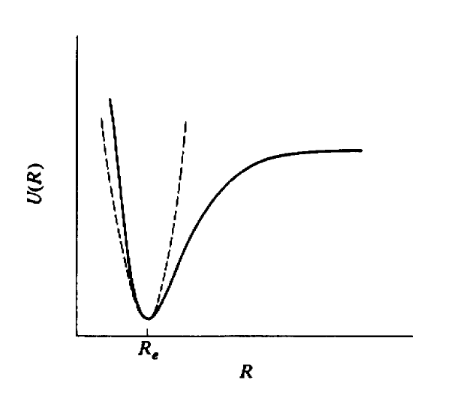
\includegraphics[width=0.8\textwidth]{curva_potencial.png}
\caption{Aproximación del potencial U(R) a una parábola (línea discontínua). Podemos observar que para distancias lejanas a la posición de equilibrio la parábola deja de ser una buena aproximación.}
\label{potencial}
\end{figure}
Realizamos ahora el cambio de variable 
\begin{equation}
q \equiv R-R_e
\end{equation}
Y definimos 
\begin{equation}
k_e \equiv	U''(R_e)
\end{equation}
El potencial queda como
\begin{equation}
U \approx U(R_e)+\frac{1}{2}k_eq^2
\end{equation}
y la ecuación de Schrödinger
\begin{equation}
-\frac{\hbar^2}{2\mu}G''(q)+\left[\frac{J(J+1)\hbar^2}{2\mu (q+R)^2}+U(R_e)+\frac{1}{2}k_eq^2-E\right]G(q)=0
\end{equation}
Escribimos ahora
\begin{equation}
\frac{J(J+1)\hbar^2}{2\mu (q+R)^2}=\frac{J(J+1)\hbar^2}{2\mu R_e^2}\left[1-2\frac{q}{R_e}+3\frac{q^2}{R_e^2}-...\right]
\end{equation}
despreciando los términos entre paréntesis y llamando 
\begin{equation}
W \equiv	E-U(R_e)-\frac{J(J+1)\hbar^2}{2\mu R_e^2}
\end{equation}
llegamos a la ecuación
\begin{equation}
-\frac{\hbar^2}{2\mu}G''(q)\left[\frac{1}{2}k_eq^2-W\right] G(q)=0
\end{equation}
que es la ecuación de Schrödinger para un oscilador armónico en una dimensión. Por tanto
\begin{equation}
W=\left(v+\frac{1}{2}\right)h\nu_e
\end{equation}
\begin{equation}
E=U(R_e)+\left(v+\frac{1}{2}\right)h\nu_e+J(J+1)hB_e
\end{equation}
con
\begin{equation}
B_e \equiv	\frac{h}{8\pi^2I_e}, \qquad I_e\equiv \mu R_e^2
\end{equation}
La vibración molecular es mucho más rápida que la rotación molecular, por lo que podemos usar la separación internuclear media $R_e$ para el cálculo del momento rotacional de inercia.
$U_e$ es la energía electrónica de la molécula, cuyo valor es
\begin{equation}
U_e \equiv	U(R_e)=E_{el} +\frac{Z_aZ_be^2}{R_e}
\end{equation}
Por tanto, vemos que podemos separar las energías de la molécula
\begin{equation}
E_{tot} = U_e+E_{vib}+E_{rot}+E_{trans}
\end{equation}
La separación entre niveles energéticos electrónicos es mucho mayor que la separación entre niveles vibracionales, la cual a su vez son mucho mayor que la separación entre niveles rotacionales.\\

La aproximación de Born-Oppenheimer permite separar la función de onda molecular en un producto de la función de onda enectrónica por la función de onda nuclear. En el tratamiento que hemos hecho de la ecuación de Schrödinger para moléculas diatómicas hemos conseguido separar la función de onda nuclear en un producto de la función de onda rotacional por la vibracional y por la translacional:
\begin{equation}
\psi=\psi_{el}\psi_{vib}\psi_{rot}\psi_{trans}
\end{equation}

Mientras que para moléculas diatómicas la interacción vibración-rotación añade sólamente pequeñas correcciones a la energía, para muchas moléculas poliatómicas la interacción vibración-rotación trae correcciones relativamente grandes. Estos nuevos términos son los llamados términos de anarmonicidad y, en moléculas diatómicas, se pueden añadir perturbativamente para ser más precisos en la descripción.\\

Otra mejora en la descripción de nuestro sistema es el uso de otras energías potenciales para $U(R)$. Previamente hemos expandido la energía potencial $U(R)$ en series en torno a $R_e$. Esta aproximación es buena para regiones cerca del equilibrio. Sin embargo, para valores grandes de $R$, la serie de Taylor en torno a $R_e$ es divergente. Una opción es tomar energías potenciales empíricas. Estos potenciales son específicos para cada estado molecular y para cada molécula. Uno de los potenciales que mejor resultados da es la función de morse, la cual tiene la forma:
\begin{equation}
U=D_e \left[ 1- e^{-a(R-R_e)} \right]^2
\end{equation}
Donde los parámetros $D_e$, $a$ y $R_e$ se obtienen experimentalmente.\\

El acoplamiento de los movimientos rotacional y vibracional en una molécula se puede entender en términos de física clásica. Sin embargo, podemos ignorar este acoplamiento y considerar la excitación de una molécula diatómica en la primera aproximación como simplemente la suma de la excitación del oscilador armónico y del rotor rígido. En ese caso obtenemos los niveles energéticos:
\begin{equation}
E(v,J)=\hbar\nu(v+\frac{1}{2})+ BhJ(J+1)
\end{equation}
Donde  las transiciones púramente rotacionales $(\Delta v = 0, \,\ \Delta J = \pm 1)$ están permitidas, pero las transiciones púramente vibracionales $(\Delta v = \pm 1, \,\ \Delta J = 0)$ no lo están. Esto se puede entender desde un punto de vista clásico. Como los movimientos vibracionales son mucho más rápidos que los movimientos rotacionales, el rotor ve una distancia internuclear $\braket{R}$, la cual es la distancia media entre los átomos. En el caso del oscilador anarmónico la distancia internuclear media $\braket{R}$ aumenta al aumentar sus números cuántico, lo que conlleva un cambio en la velocidad de rotación. La regla de selección $\Delta J=0$ solo es válida cuando el momento angular de la molécula es paralelo al eje de su cilindro.
En la figura (\ref{transiciones}) se observan las líneas típicas para un potencial de morse.
\begin{figure}
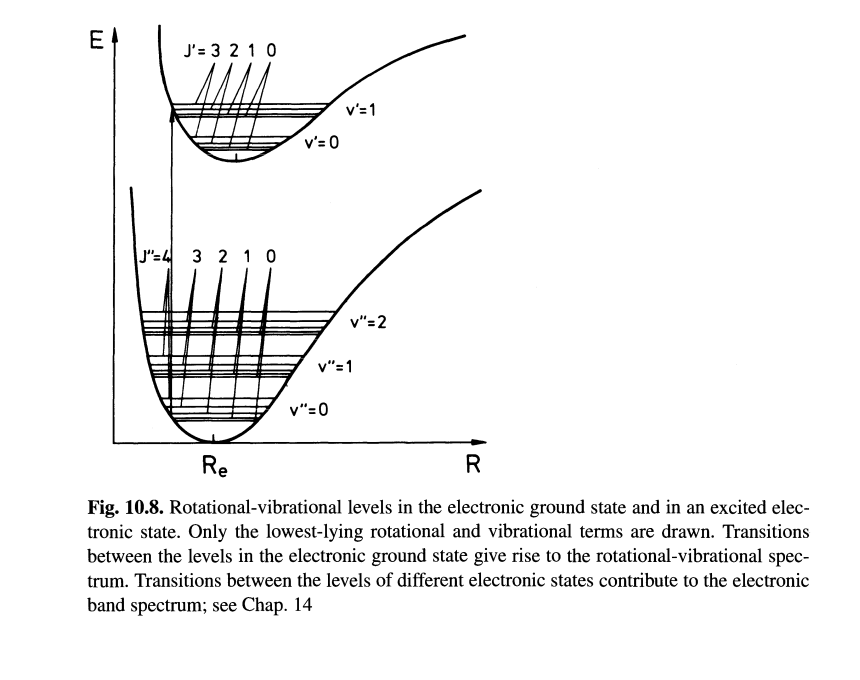
\includegraphics[width=0.8\textwidth]{niv_rot_vib_elect.png}
\caption{Niveles vibracionales-rotacionales en el estado electrónico fundamental y en un estado electrónico excitado. Las transiciones entre niveles en el estado electrónico fundamental dan lugar al espectro vibracional-rotacional. Las transiciones entre estados electrónicos diferentes contribuyen al espectro de la banda electrónica}
\label{transiciones}
\end{figure}
\newpage
\printbibliography
\end{document}

